\section{Results}
\label{sec:results}

\subsection{Validity and discarded shared structure}

All 24 registered cases completed at the substantive 4,000-world scale. The
largest observed joint-linear true-null family rejection rate among the 23
valid-model cases is \MaxValidJointFWER\%, below the nominal 5\% ceiling.
This checks the implemented model; the proof remains conditional on
Section~\ref{sec:methods}. No calibration-envelope failure was observed in
those cases. Zero out of 4,000 has a Wilson upper limit of \ZeroWilsonUpper\%
within each case, not zero failure probability or simultaneous coverage across
cases. No stored crossing-inclusion violation was recorded.

Figure~\ref{fig:power} compares matched methods on the same worlds. At effect
0.05 and equal turnover, joint first-stream power is \EqualPowerJoint\%
[\EqualJointLower\%, \EqualJointUpper\%], versus \EqualPowerSeparate\%
[\EqualSeparateLower\%, \EqualSeparateUpper\%] for separate bounds.
The paired improvement is \EqualPowerGain\ percentage points
[\EqualGainLower, \EqualGainUpper], using a Wilson interval for the joint-only
rejection event. Joint and known-cost oracle results coincide because the
common coefficient cancels exactly.

At half overlap, joint/separate powers are \HalfPowerJoint\%/\HalfPowerSeparate\%.
At zero reference turnover their proxies coincide. At effect 0.02, even perfect
cancellation gives only 7.325\% joint power; at effect 0.005 it is 0.475\%.
With 512 initial calibration observations, half-overlap joint/separate powers
rise to 74.925\%/18.425\%. Both calibration quality and uncertainty geometry
matter. These scale-dependent results do not demonstrate generally powerful
strategy discovery or estimate real trading fees.

\begin{figure}[tbp]\centering
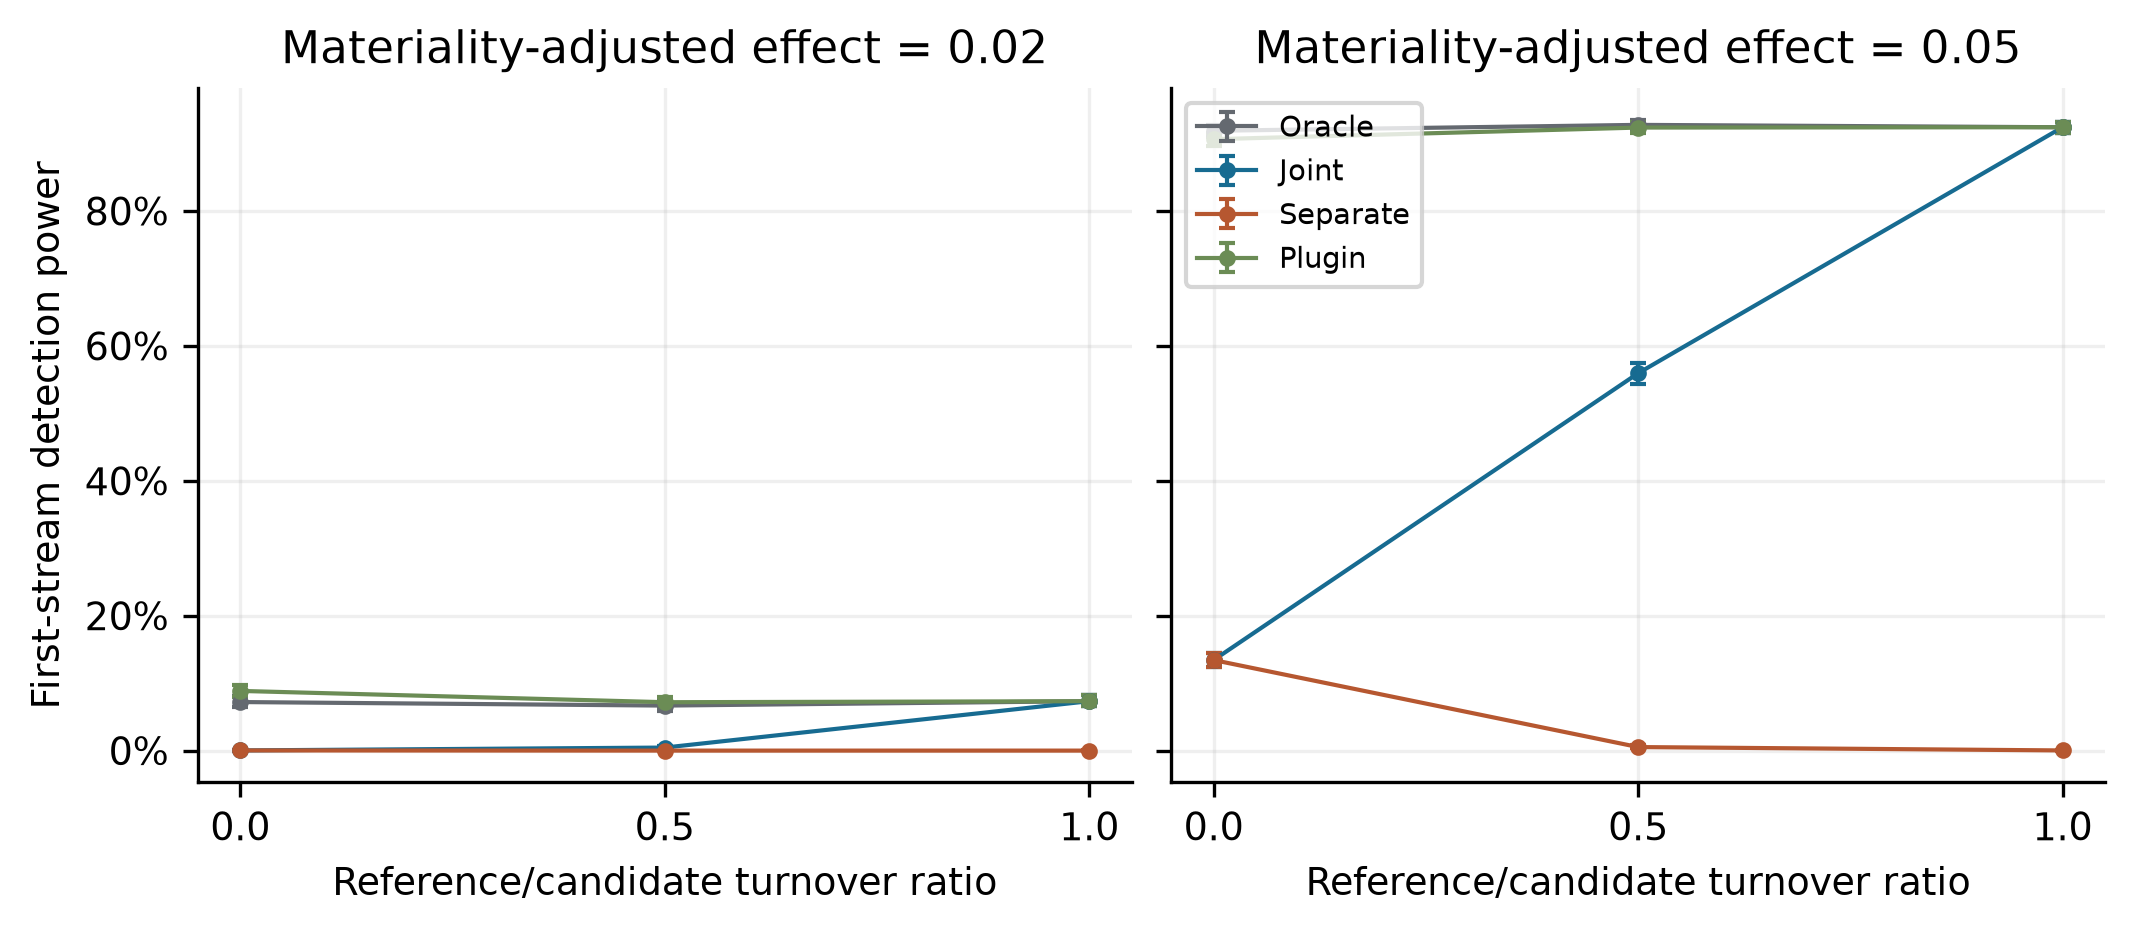
\includegraphics[width=\textwidth]{generated/simulation-power.png}
\caption{Overlap/effect comparison with 95\% Wilson intervals over independent
worlds. Methods within a case use paired data. Plugin is unguaranteed. Lines
connect three evaluated points; overlap cases use separate seeds.}\label{fig:power}
\end{figure}

The invalid symmetric-upper rule gives \UpperBothFWER\% false family rejection
[\UpperNullLower\%, \UpperNullUpper\%] when the reference trades more
(Figure~\ref{fig:validity}). A conservative cost convention for each portfolio
is therefore not necessarily conservative for their difference. Under the
explicitly invalid cost-shift law, every world's envelope eventually fails
and plugin false rejection is \PluginDriftFWER\%
[\PluginDriftLower\%, \PluginDriftUpper\%]. Low joint rejection in that
particular violation case does not restore its missing stationarity guarantee.

All four Hoeffding, fixed-time and peeked controls have zero rejections in every
case. Their support bound and the chosen signal/noise scale are too conservative
to provide an informative empirical optional-stopping comparison. These results
do not demonstrate peeking inflation, and absence of observed inflation does
not validate peeking. Appendix~\ref{app:counterexamples} addresses separate
invalidity mechanisms exactly, without substituting a favorable new simulation.

\begin{figure}[tbp]\centering
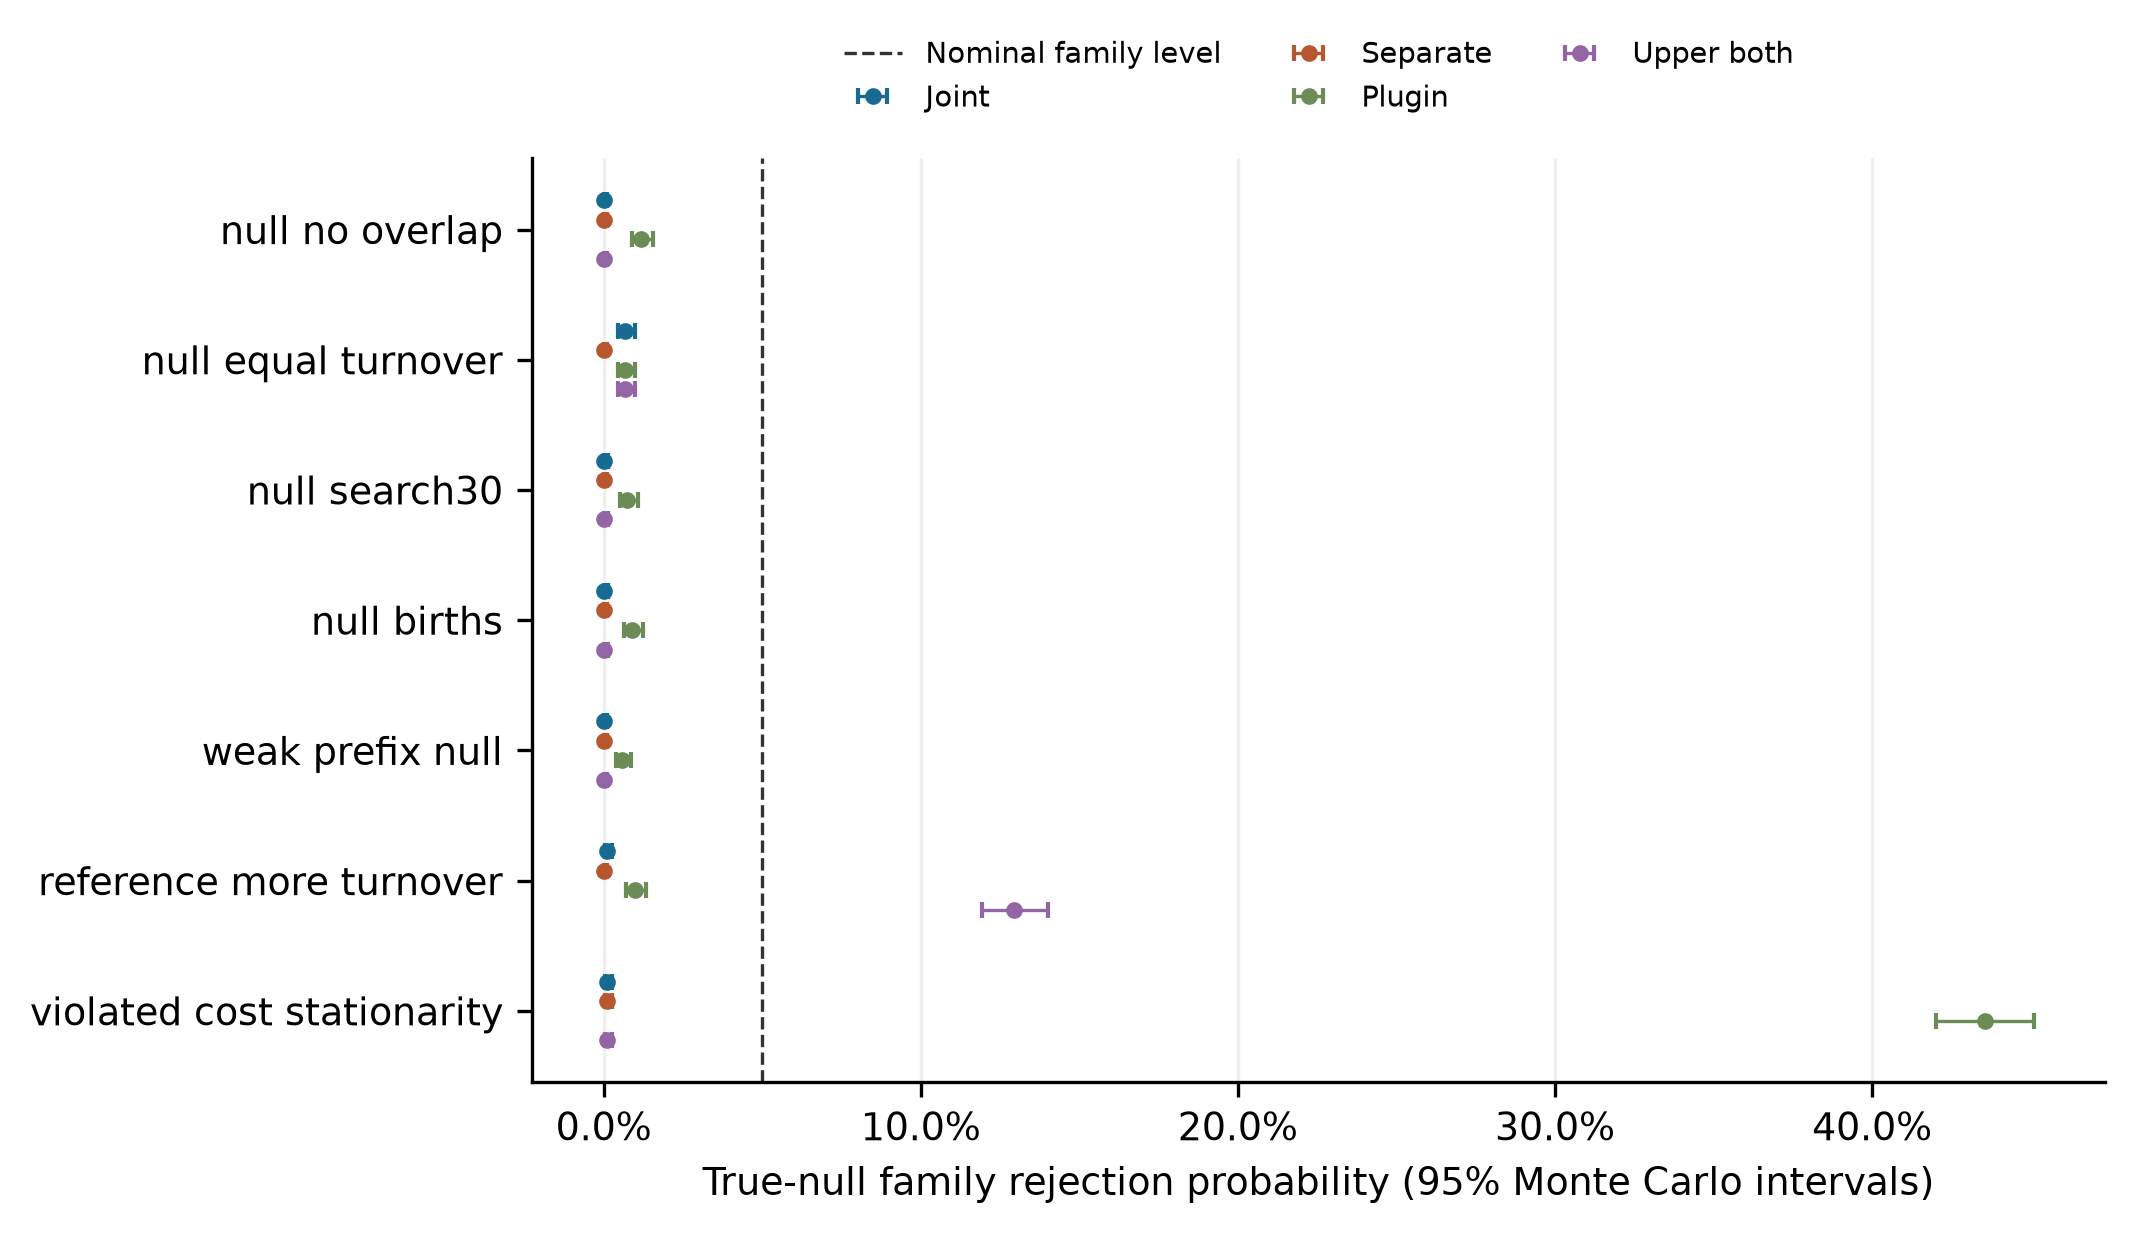
\includegraphics[width=\textwidth]{generated/simulation-validity.png}
\caption{Selected null diagnostics; the supplement retains every method/case.
The final row violates stationary calibration. Upper both and Plugin have no
asserted guarantee. Zero estimates retain nonzero Wilson upper bounds. The
dashed line is the declared 5\% family level.}\label{fig:validity}
\end{figure}

\subsection{Timing, utility and computation}

Equal-turnover joint restricted first-alternative detection time is 298.3
calendar steps versus 799.9 for separate bounds. The paired mean paper-utility
difference is 24.946 synthetic units [24.650,25.242], an approximate normal
Monte Carlo interval. This reflects the registered allocation rule and effect,
not dollars, compounded wealth, actual execution quality or general optimality
(Figure~\ref{fig:utility}).

Delay reduces matured labels from 800 to 160 and calibration opportunities,
so the lower power does not isolate delay alone. Birth cases change the family
from ten streams to five, give the first birth a larger allowance (0.02 versus
0.004), and stagger observation counts. Higher first-stream power cannot be
attributed solely to adaptation or prescreening. Within-case joint/separate
contrasts remain paired.

Case runtimes sum to 2,715.6 seconds with concurrent local work; this is a
recorded-host observation, not a controlled speed benchmark. Mixture-array
bytes are reported separately from whole-process peak memory, which was not
measured. Saved worlds support independent truth-mask, crossing-time, summary
and activation checks. Per-trial latent trajectories require the frozen
generator and seed; they are not stored in the final world arrays.

\begin{figure}[tbp]\centering
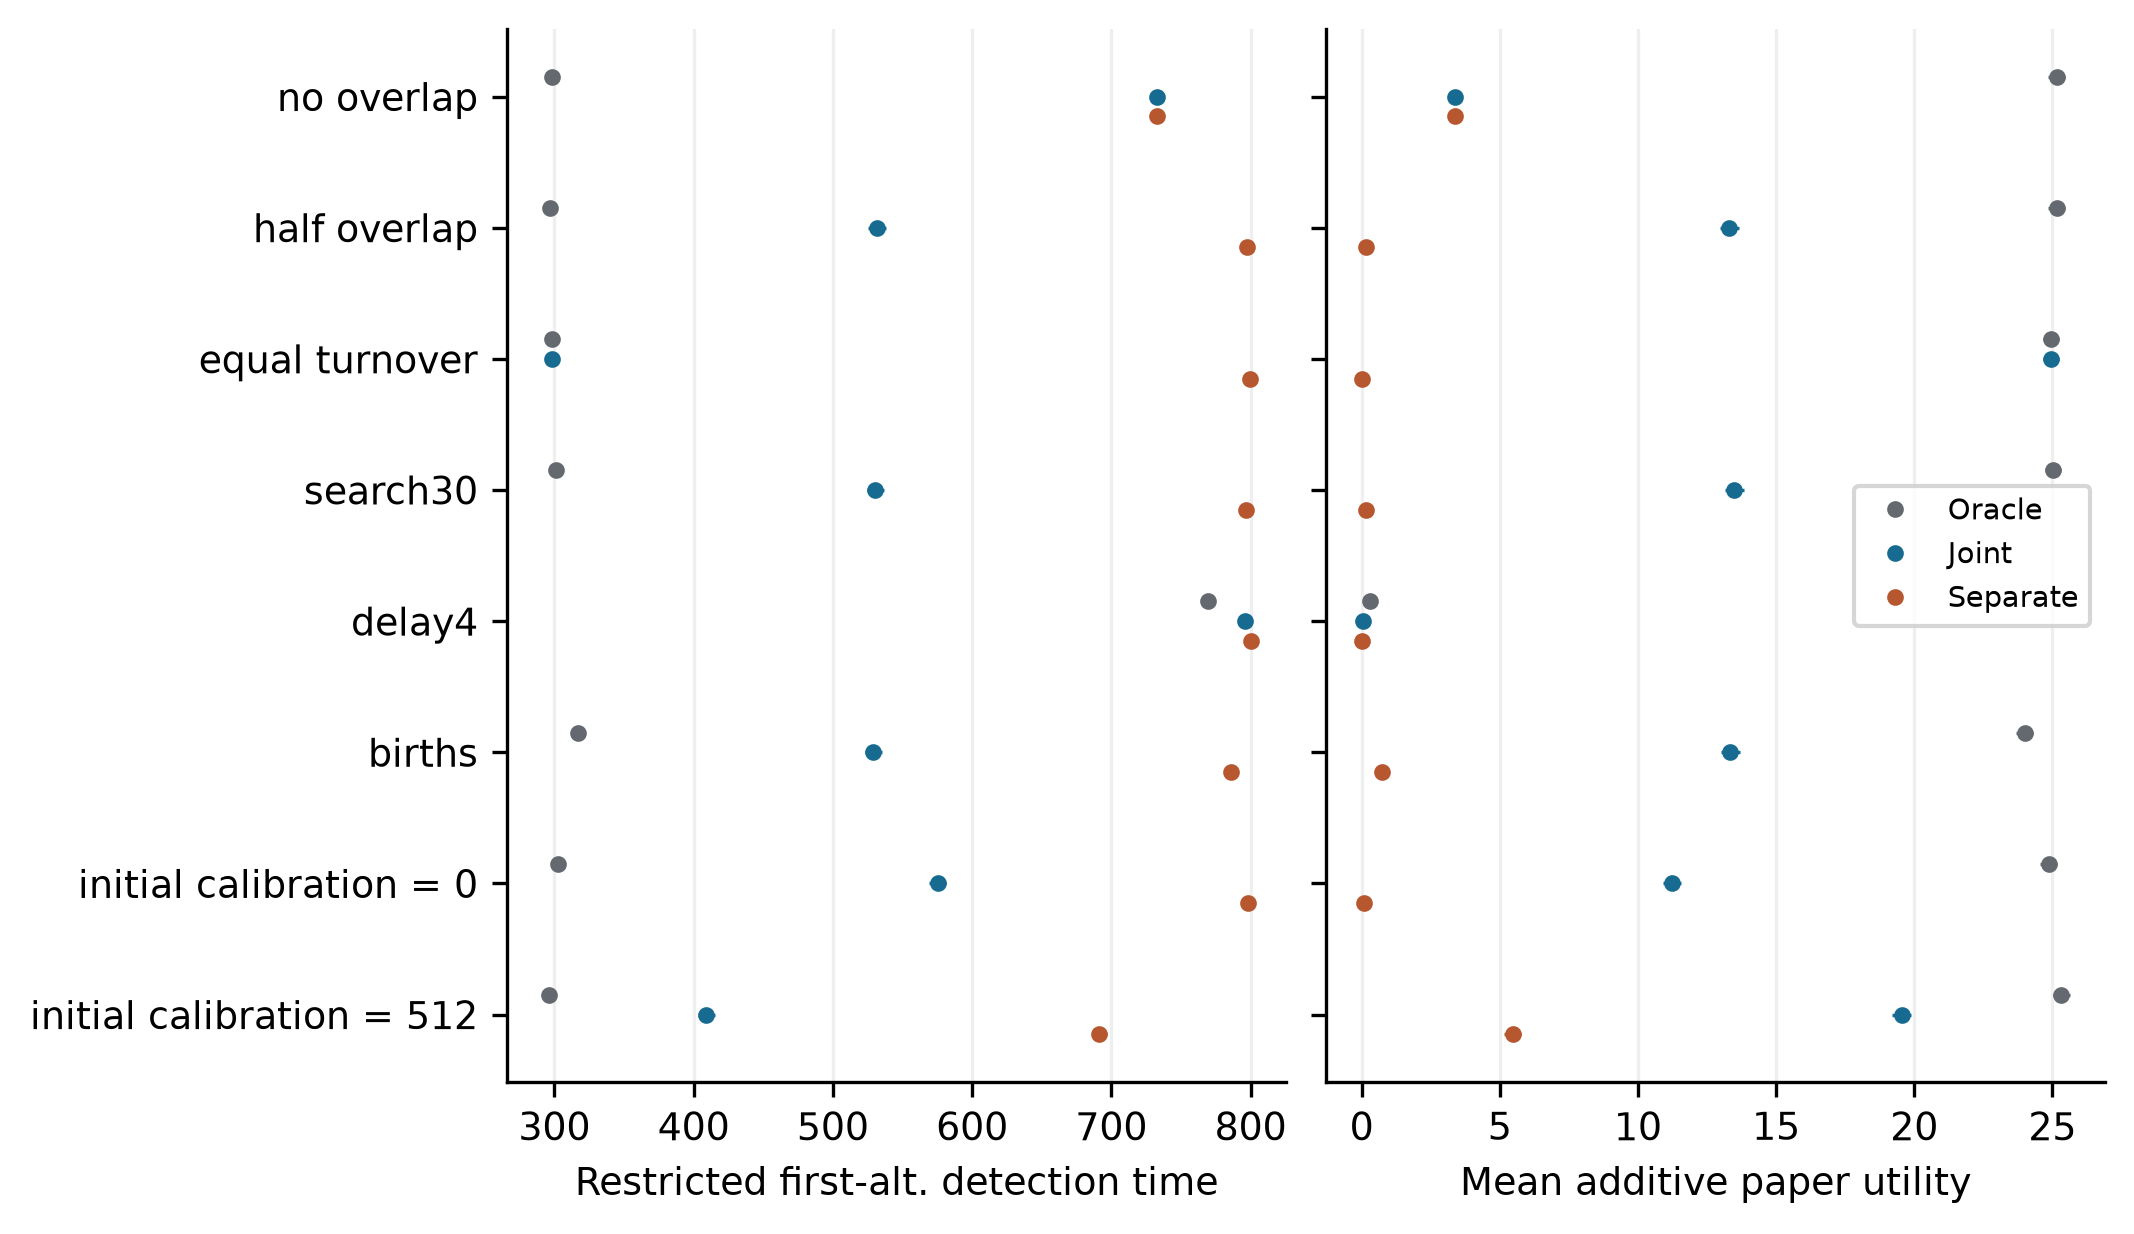
\includegraphics[width=\textwidth]{generated/simulation-delay-utility.png}
\caption{Effect-0.05 diagnostics. Time is first any-alternative discovery from
origin, horizon-censored; Figure~\ref{fig:power} reports first-stream power.
Approximate Monte Carlo intervals are omitted for degenerate samples.
Between-case comparisons change several design factors.}\label{fig:utility}
\end{figure}

\subsection{Separating evidence form from temporal cost pessimism}
\label{sec:followup-results}

All 25 separately frozen follow-up cases completed at 4,000 worlds and 800
labels. Across method/case combinations within their stated null scope, the
largest observed true-null family rejection rate is
\FollowupSupportedMaxNullRate\%. No used cost-envelope failure or interval
conflict was observed. These frequencies support the implementation checks;
they do not establish sharpness of the nominal 5\% bound. The calibration
spending rule is deliberately conservative, and neither cases nor comparators
constitute one jointly controlled family of research conclusions.

Figure~\ref{fig:followup-power} displays all eight prespecified effect-0.05
factorial cells. With high volatility, fixed cost information and alternating
turnover differences, coherent EB has \FollowupStaticAltCoherent\% first-stream
power versus \FollowupStaticAltLocal\% for local joint EB. With contracting
information these become \FollowupContractAltCoherent\% and
\FollowupContractAltLocal\%. The paired contrasts in
Table~\ref{tab:followup-paired} retain their Monte Carlo uncertainty. In the
low-volatility fixed/alternating cell, the coherent/local difference reaches
\FollowupCoherentGainMax\ percentage points. Thus a local robust calculation
can discard much of the available evidence even when its per-label cost
geometry is correct. The static, one-sign controls show zero observed
coherent/local gain. This is an observed property of these controls, not a
general EB equality: the adverse endpoint of a nonmonotone factor can change
across labels.

\begin{figure}[tbp]\centering
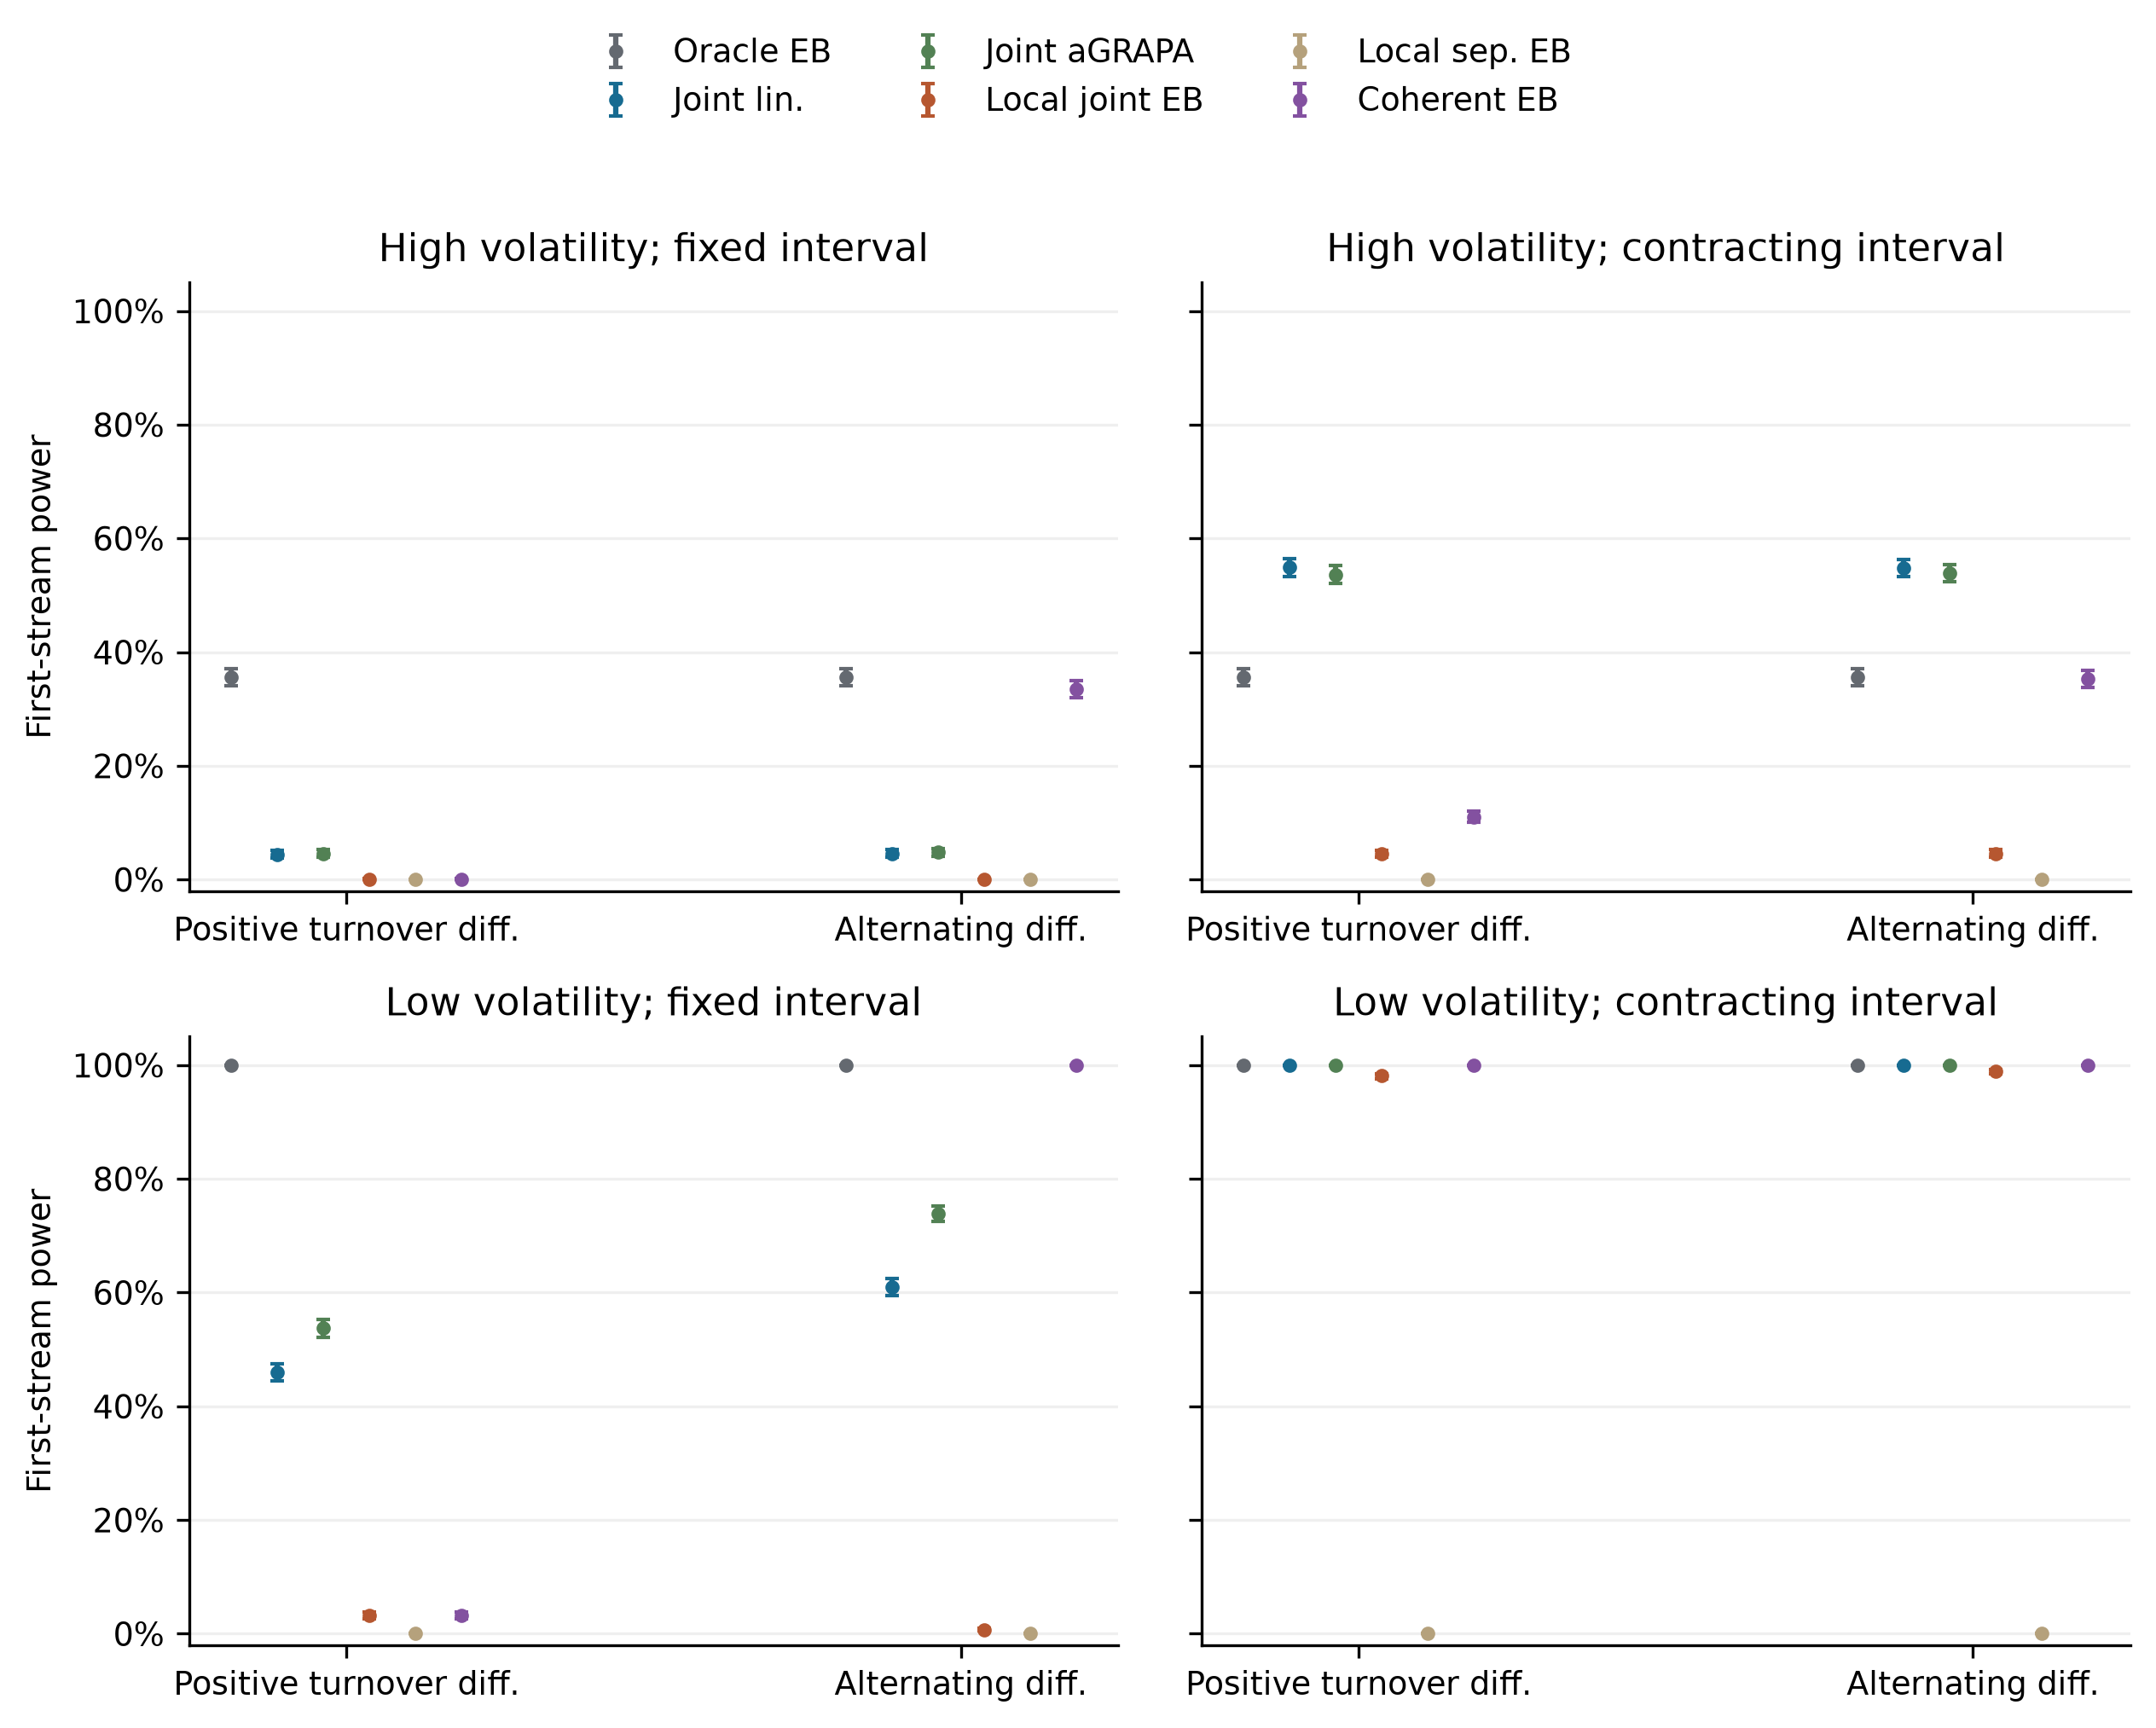
\includegraphics[width=\textwidth]{generated/followup/power.png}
\caption{Follow-up effect-0.05 factorial comparison. Points have within-case
95\% Wilson intervals over 4,000 worlds. Oracle EB knows the true cost;
its predictable centers match the other EB methods. Static and contracting
information use different calibration schedules. Factorial cells share seeded
innovations and must not be pooled as independent replications.}
\label{fig:followup-power}
\end{figure}

Temporal coherence does not make EB uniformly preferable to other evidence
forms. Under high volatility and contracting information, joint linear betting
has greater power than coherent EB, for both turnover patterns. Lower volatility
and sign changes can reverse that comparison. Likewise, the joint aGRAPA minus
joint linear power contrast ranges from \FollowupAgraGainMin\ to
\FollowupAgraGainMax\ percentage points across the eight primary cells. Its
negative high-volatility/contracting contrasts and positive low-volatility/static
contrasts rule out a uniform empirical advantage. Predictable refitting also
has a stronger conditional-null requirement than the fixed-grid comparisons.

Local joint versus local separate EB gains range from
\FollowupJointSeparateGainMin\ to \FollowupJointSeparateGainMax\ percentage
points. These are a different ablation from coherent versus local joint EB.
Both must be held separate from changing the underlying betting rule or the
cost-calibration schedule. The results identify mechanisms within the declared
synthetic family, rather than a universally best sequential procedure.

Weak effects remain difficult. Across the eight effect-0.02 cells, coherent EB
first-stream rejection never exceeds 1.825\%. The stronger effect-0.05 gains
therefore do not establish sensitive detection of small improvements at this
horizon, even inside the synthetic family.

\begin{table}[tb]\centering
\begingroup\small\setlength{\tabcolsep}{3pt}
\begin{tabular}{lrrr}\toprule
Case & aGRAPA - linear & Coherent - local EB & Joint - separate EB\\\midrule
F03 & 0.12 [-0.20, 0.45] & 0.00 $^{\ddagger}$ & 0.03 [-0.02, 0.07]\\
F06 & 0.18 [-0.15, 0.50] & 33.50 [32.04, 34.96] & 0.00 $^{\ddagger}$\\
F09 & -1.23 [-1.85, -0.60] & 6.48 [5.71, 7.24] & 4.50 [3.86, 5.14]\\
F12 & -0.88 [-1.50, -0.25] & 30.73 [29.30, 32.15] & 4.60 [3.95, 5.25]\\
F15 & 7.72 [6.90, 8.55] & 0.00 $^{\ddagger}$ & 3.20 [2.65, 3.75]\\
F18 & 12.90 [11.86, 13.94] & 99.30 [99.04, 99.56] & 0.70 [0.44, 0.96]\\
F21 & 0.00 $^{\ddagger}$ & 1.90 [1.48, 2.32] & 98.10 [97.68, 98.52]\\
F24 & 0.00 $^{\ddagger}$ & 1.10 [0.78, 1.42] & 98.90 [98.58, 99.22]\\
\bottomrule\end{tabular}
\endgroup
\caption{Prespecified effect-0.05 contrasts in first-stream power, in percentage points. Intervals are paired, approximate, unadjusted 95\% normal Monte Carlo intervals across worlds. $^{\ddagger}$ marks a degenerate sample with an unavailable normal interval, not known zero uncertainty. Case definitions appear in the supplement.}\label{tab:followup-paired}
\end{table}


\begin{figure}[tbp]\centering
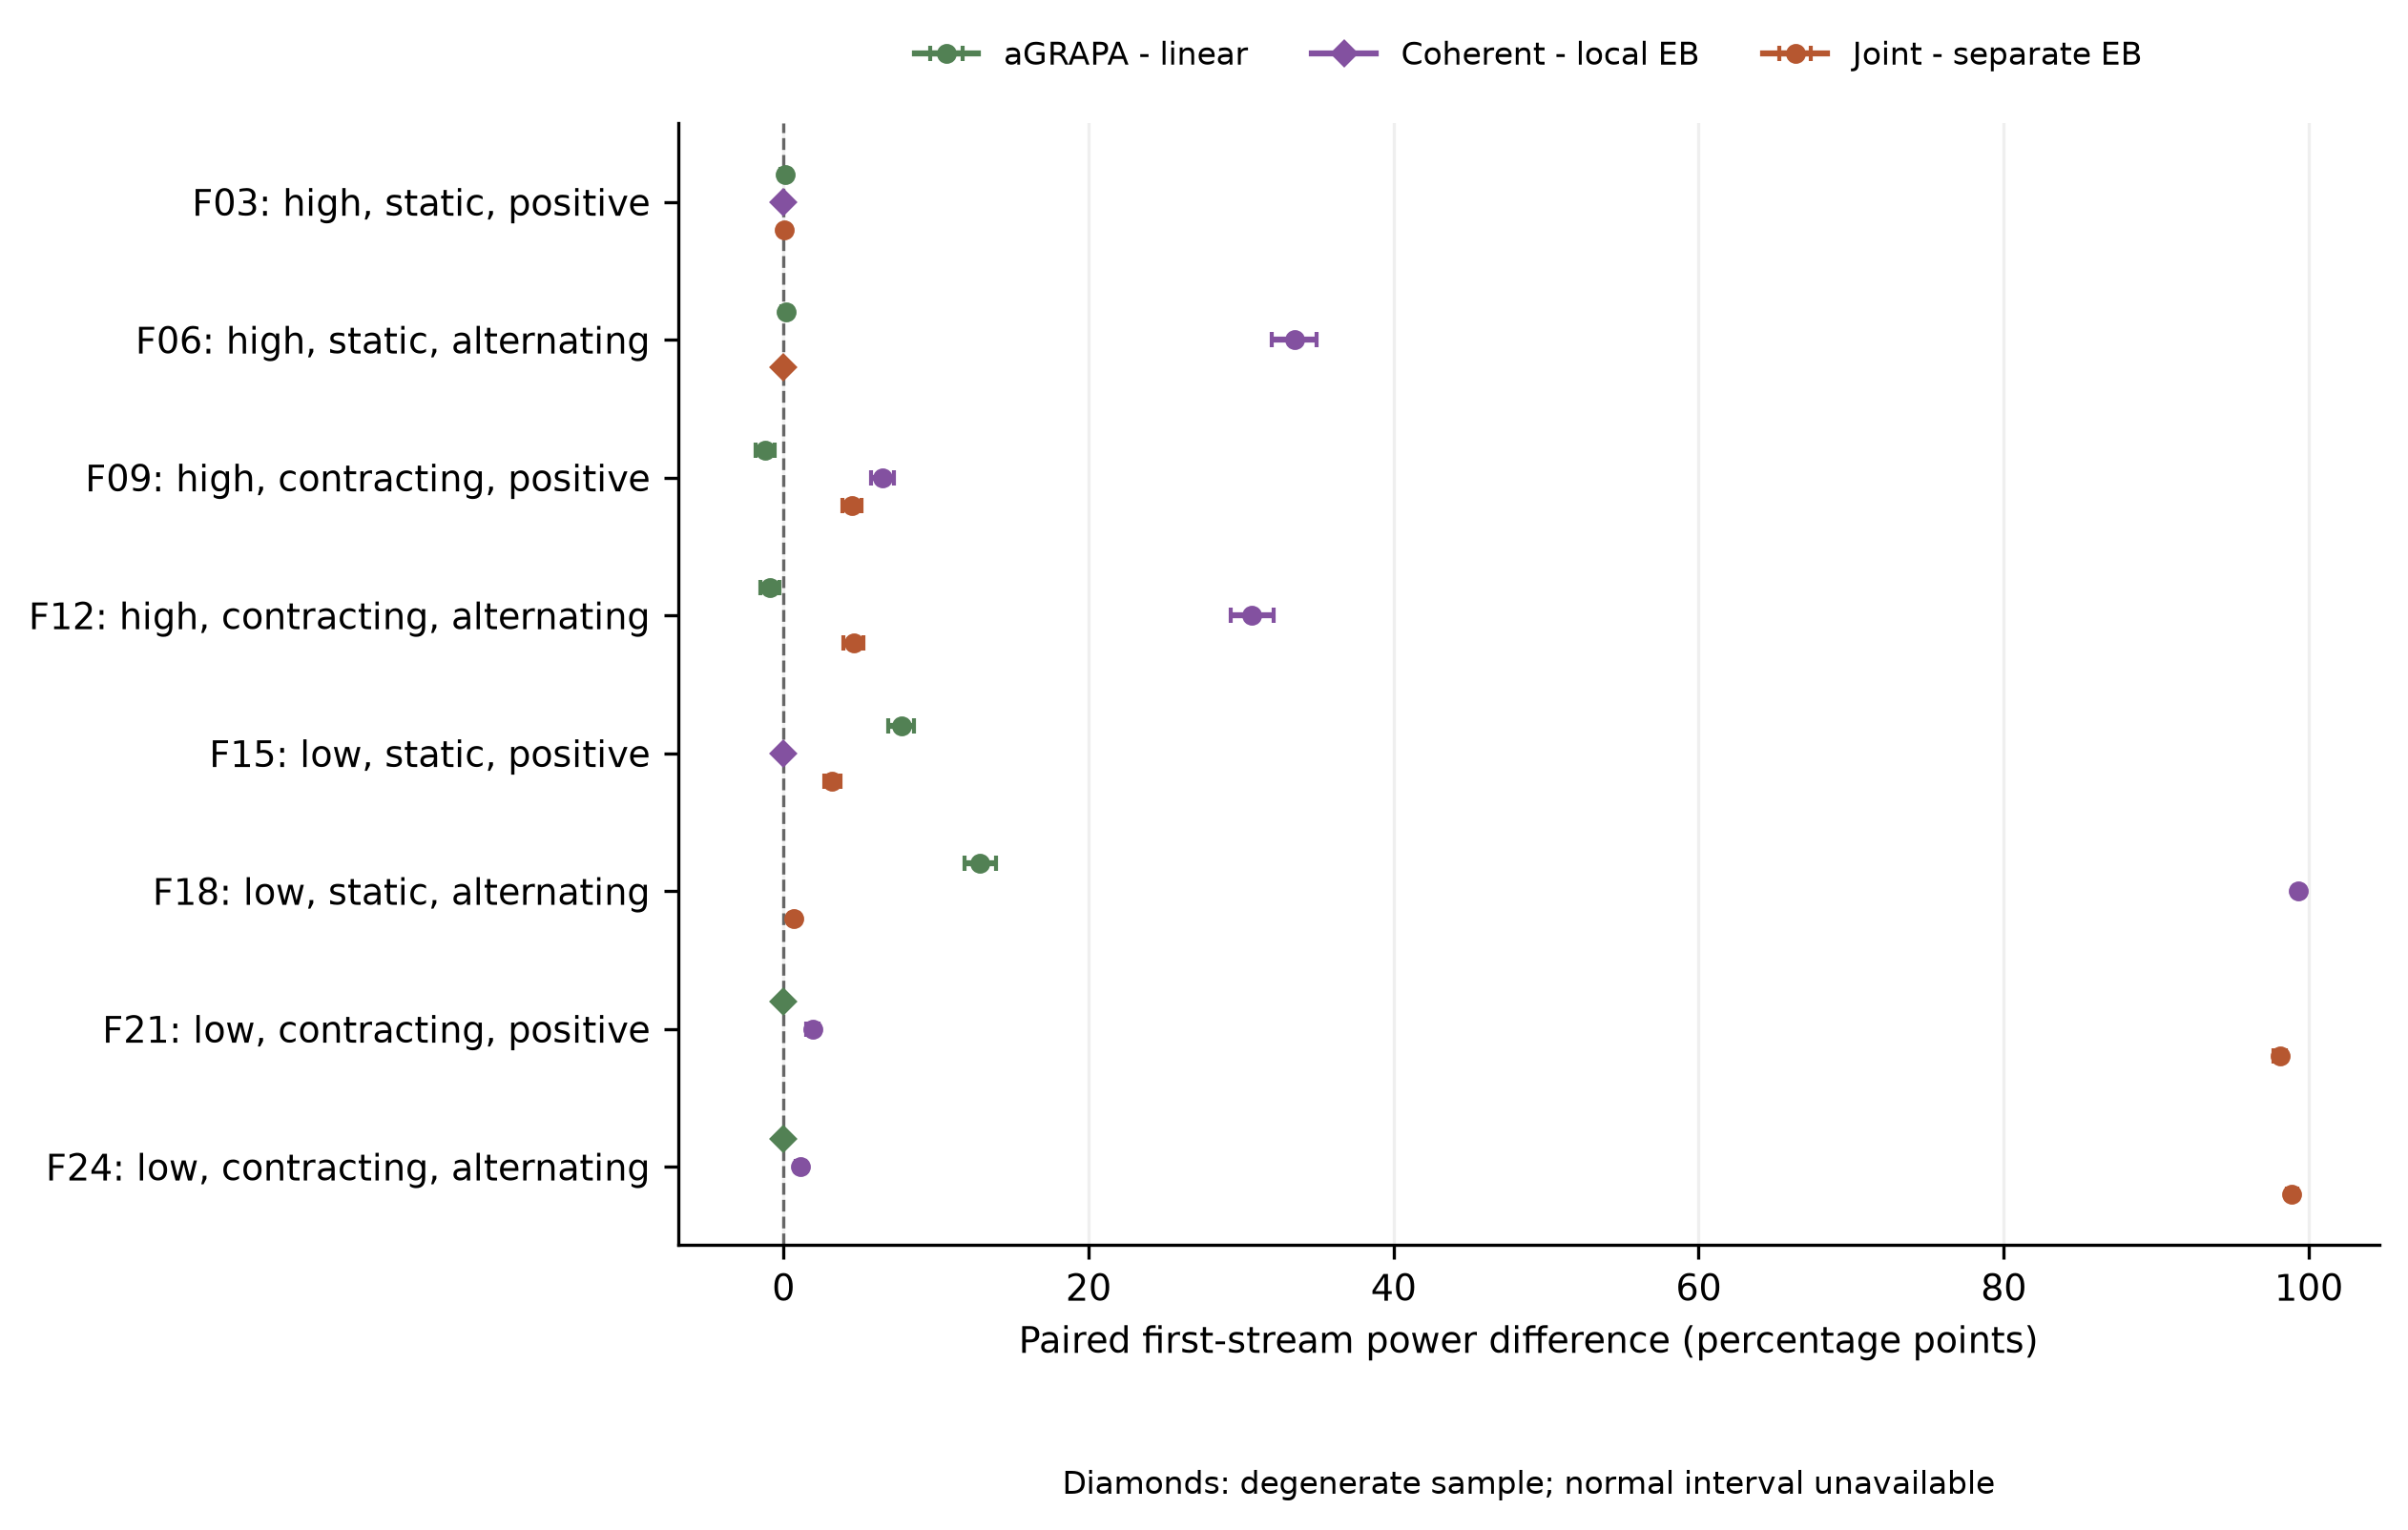
\includegraphics[width=\textwidth]{generated/followup/paired-power.png}
\caption{The three primary within-case ablations, with paired approximate
95\% normal Monte Carlo intervals. Intervals are unadjusted descriptive
summaries; diamonds denote degenerate samples for which that normal interval
is unavailable. Every registered contrast, including weaker effects, is
retained in the machine-readable supplement.}
\label{fig:followup-paired}
\end{figure}

Restricted detection time and subsequent paper utility follow the same
implementation's recorded allocation rule, not a funded portfolio. Saturated
end-of-horizon power does not imply identical detection times or utility;
those endpoints remain in the complete result tables. The prefix-weak diagnostic
has no first-stream rejections for any method. Its family rejection counts are
one for oracle linear, two for oracle aGRAPA and zero for the other methods,
out of 4,000 worlds each. These low frequencies do not validate aGRAPA
under that weaker null: Section~\ref{sec:followup-methods} gives its scope and
a deterministic counterexample to general predictable refitting.

Case kernels total 2,542.6 seconds on the recorded host. Named persistent state
uses 24,220,080 bytes per case; this is not peak process memory and runtime
excludes serialization. These observations describe reproducibility costs,
not controlled speed comparisons. All 250 method summaries, 150 paired
contrasts, calibration diagnostics and source-linked array outputs are retained.


\subsection{No demonstrated adaptive Bitcoin edge}

The primary four-hour period has 3,948 scored candles, no missing scored
intervals and no feature pauses. The selector makes no switches. Its full
Binance history has 27 decisions, all retaining EMA 50/200. Fixed/adaptive raw
paths are exactly identical, with the same \PrimaryFixedReturn\% primary
return (Table~\ref{tab:market}). The ensemble returns \PrimaryEnsembleReturn\%.
These point estimates do not establish adjusted superiority over the controls.

\begin{table}[tbp]\centering\small
\begin{tabular}{lrrrrr}\toprule Policy & Return (\%) & Max DD (\%) & Exposure (\%) & Trades & Turnover\\\midrule
Fixed EMA 50/200 & 2.61 & -20.05 & 26.8 & 31 & 13.54\\
Adaptive & 2.61 & -20.05 & 26.8 & 31 & 13.54\\
Ensemble & -2.21 & -20.09 & 25.7 & 88 & 14.68\\
Cash & 0.00 & 0.00 & 0.0 & 0 & 0.00\\
Buy and hold & -11.27 & -53.45 & 100.0 & 0 & 0.00\\
Volatility target & -6.30 & -36.73 & 51.5 & 20 & 2.26\\
Slow resizing & 4.84 & -18.50 & 26.3 & 27 & 12.75\\
Fixed EMA 25/100 & -5.17 & -22.65 & 24.4 & 57 & 25.51\\
Fixed EMA 100/400 & -4.63 & -21.26 & 26.8 & 17 & 6.65\\
\bottomrule\end{tabular}

\caption{Primary retrospective four-hour policies at 25 bps per side. Exposure
is average closing weight; turnover sums absolute traded notional divided by
pre-trade wealth. Holdings are inherited and terminal holdings marked.}
\label{tab:market}
\end{table}

Bitstamp has two pre-window switches and different inherited wealth, but no
scored-window switches. Its rebased paths agree to floating-point precision.
Differences around $10^{-16}$ produce some raw cost-grid sign changes; these
are not economic break-even costs. A post-outcome note preserves raw artifacts
and marks per-bar differences within $10^{-12}$ as numerical identity.
Binance's zero bootstrap interval and Bitstamp's roundoff intervals resample
an identical historical difference, not a known zero future advantage.

\begin{figure}[tbp]\centering
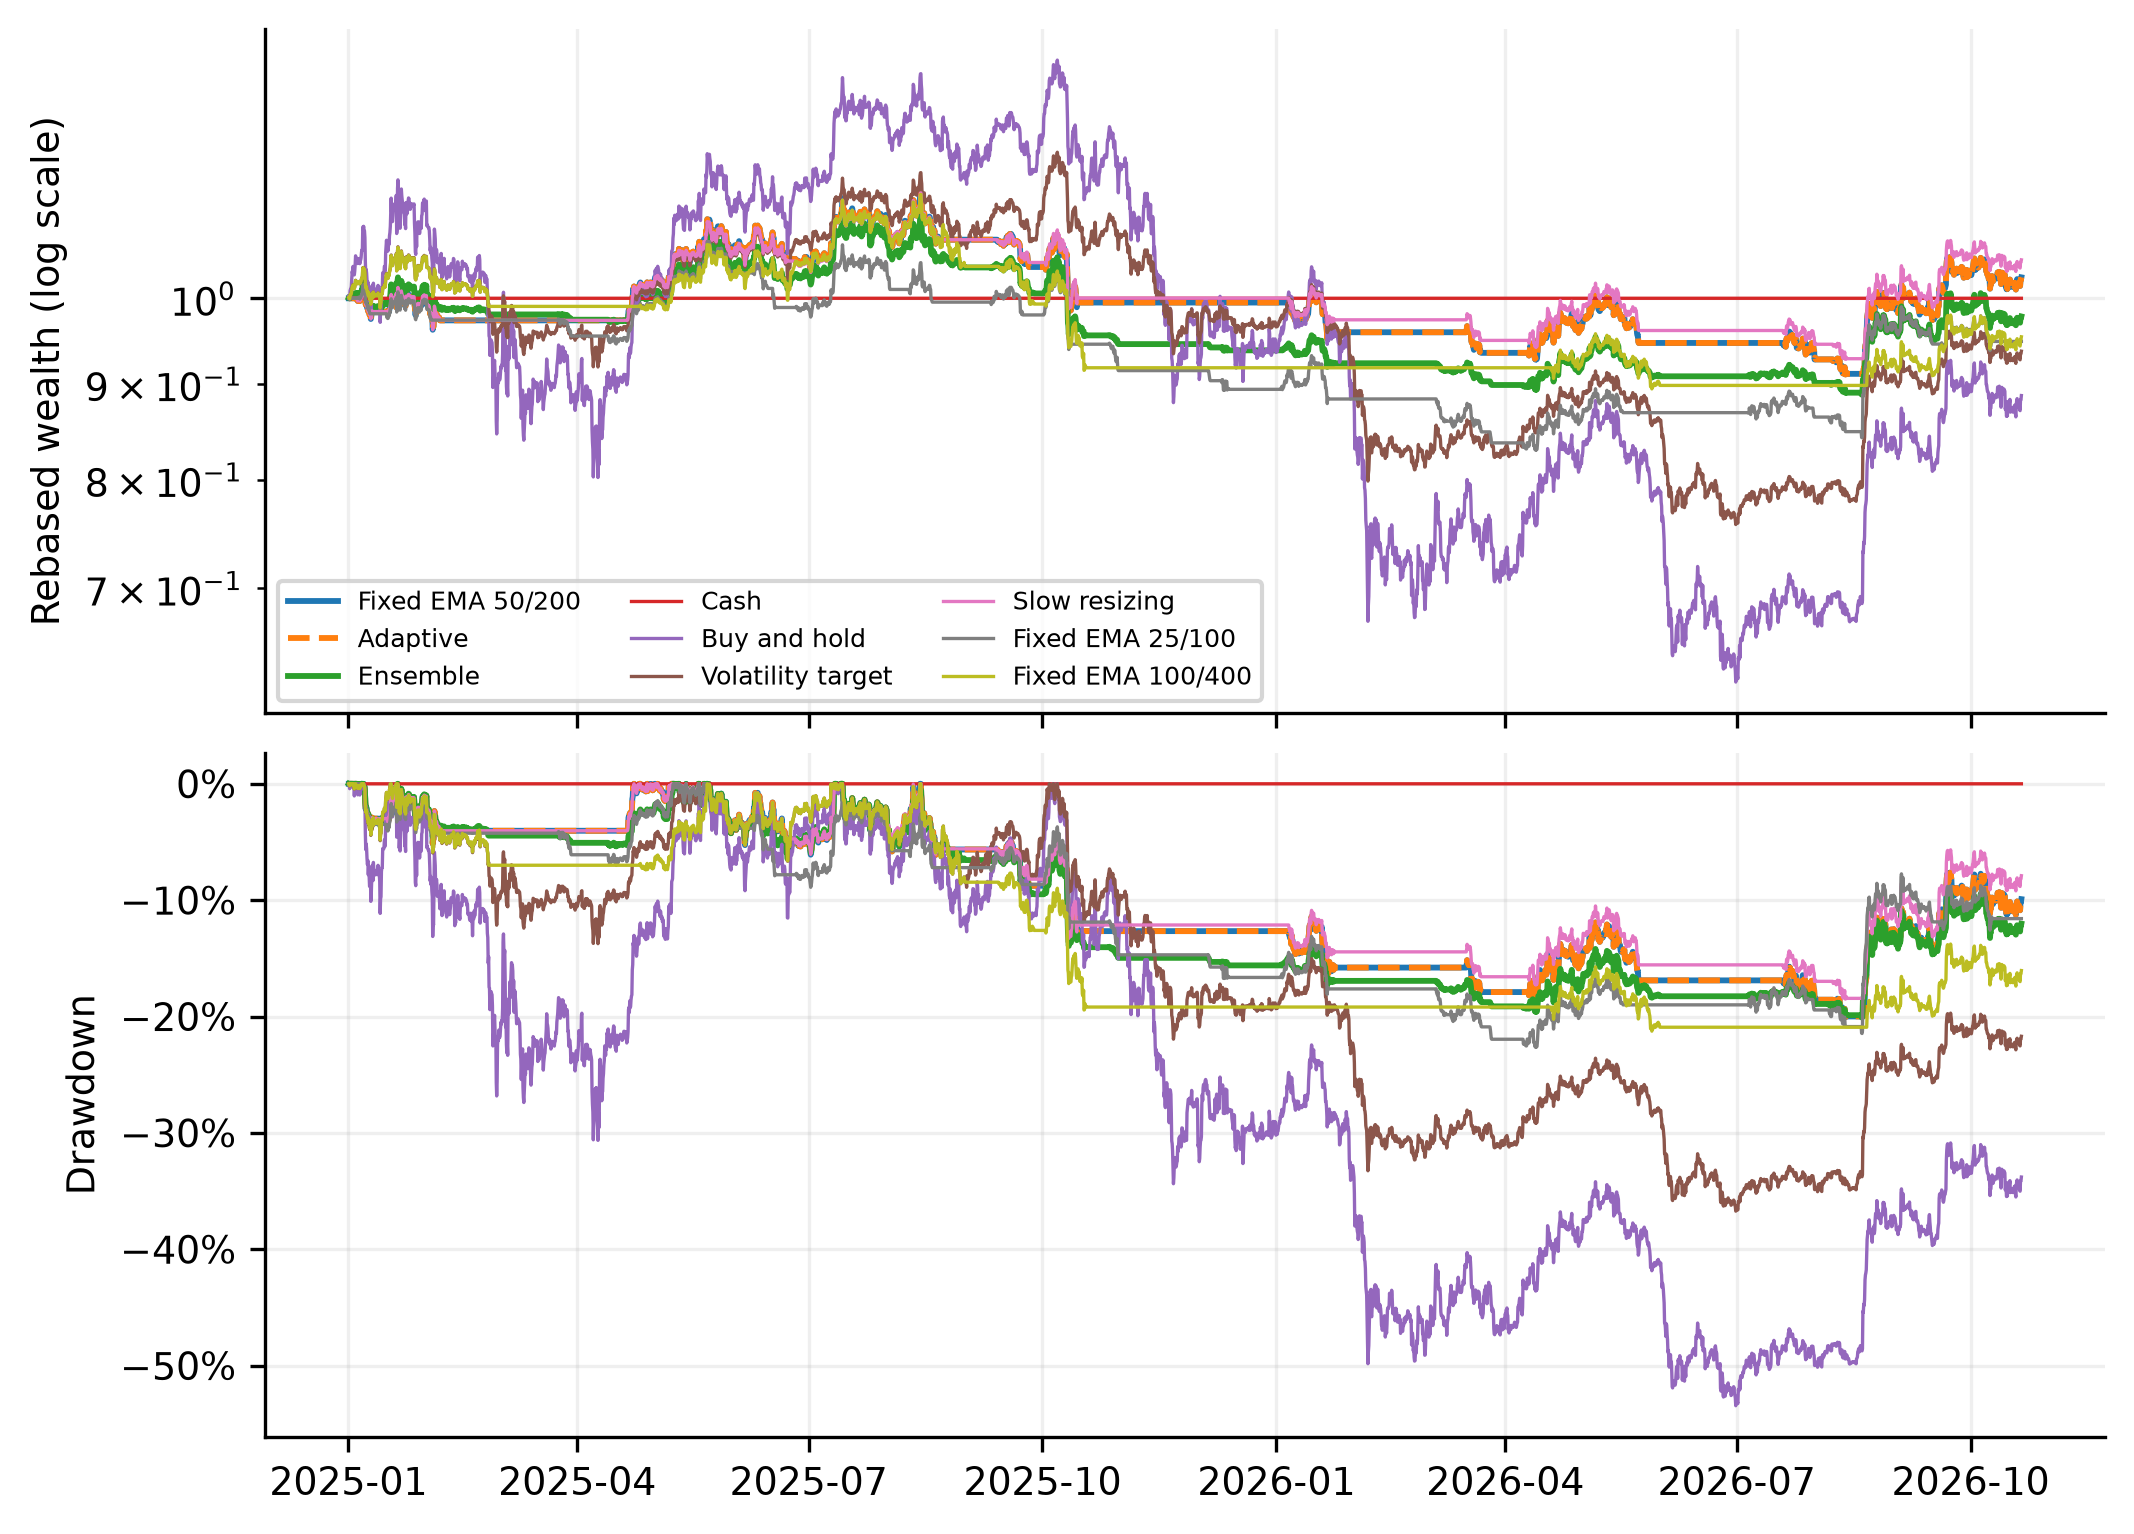
\includegraphics[width=\textwidth]{generated/market-primary-paths.png}
\caption{Primary rebased wealth and drawdown at assumed 25 bps. Adaptive and
fixed lines coincide. Passive and risk-controlled books have different
exposures; no line represents verified historical fills.}\label{fig:marketpaths}
\end{figure}

On the common 243-day window, hourly and daily adaptive annualized mean-log
differences are $-9.653\%$ and $-6.681\%$ at base cost. The hourly approximate
30-day interval is $[-32.175\%,2.610\%]$; the daily interval is
$[-22.419\%,5.042\%]$.
Both span losses and gains, including the 2\% materiality threshold. Neither
material gain nor stable loss is established. There are two hourly and three
daily switches. These are dependent market observations, not independent
replications or evidence of a universally best timeframe.

There are only 8.1 nominal 30-day blocks in this 243-day window. This does not
validate stability or finite-sample coverage. A post-outcome deterministic
diagnostic in Table~\ref{tab:blockedges} shows the finite-sample edge weighting
of the specified non-circular resampler: its expected resampled mean differs
from the observed mean. These are not new intervals, and no better-looking
correction replaces the registered percentile results.

\begin{table}[tbp]\centering\small
\begin{tabular}{lrrr}
\toprule
Case & Nominal blocks & Observed & Expected resample\\
\midrule
Hourly & 8.1 & -9.653\% & -11.150\%\\
Daily & 8.1 & -6.681\% & -7.256\%\\
\bottomrule
\end{tabular}

\caption{Primary 25 bps matched-window mean log differences, annualized linearly.
The expected resample averages exactly over all possible block starts, including
the final truncated block. Nominal block count is not an independent sample size.}
\label{tab:blockedges}
\end{table}

All five costs leave four-hour comparisons identical and hourly/daily point
estimates negative. Neither nonidentical case has a cost-grid sign-change
bracket. The hourly deficit shrinks slightly at larger costs, illustrating why
reference costs must enter the paired contrast. Direct fee-drag differences
are small relative to the hourly/daily price/holdings differences; this is
accounting description, not causal attribution. All cost/control outcomes are
retained in the supplement.

\begin{table}[tbp]\centering\small
\begin{tabular}{lrrr}\toprule Case & Annual log diff. (\%) & 30-day interval (\%) & Switches\\\midrule
Binance primary 4h & 0.00$^\dagger$ & identical path$^\dagger$ & 0\\
Binance matched 4h & 0.00$^\dagger$ & identical path$^\dagger$ & 0\\
Binance matched 1h & -9.65 & [-32.18, 2.61] & 2\\
Binance matched 1d & -6.68 & [-22.42, 5.04] & 3\\
Bitstamp primary 4h & 0.00$^\dagger$ & identical path$^\dagger$ & 0\\
Bitstamp matched 4h & 0.00$^\dagger$ & identical path$^\dagger$ & 0\\
\bottomrule\end{tabular}

\caption{Base-cost paired results. $\dagger$ denotes historical numerical
identity, not zero future uncertainty. Other intervals are approximate,
retrospective and unadjusted.}\label{tab:pairedmarket}
\end{table}

\begin{figure}[tbp]\centering
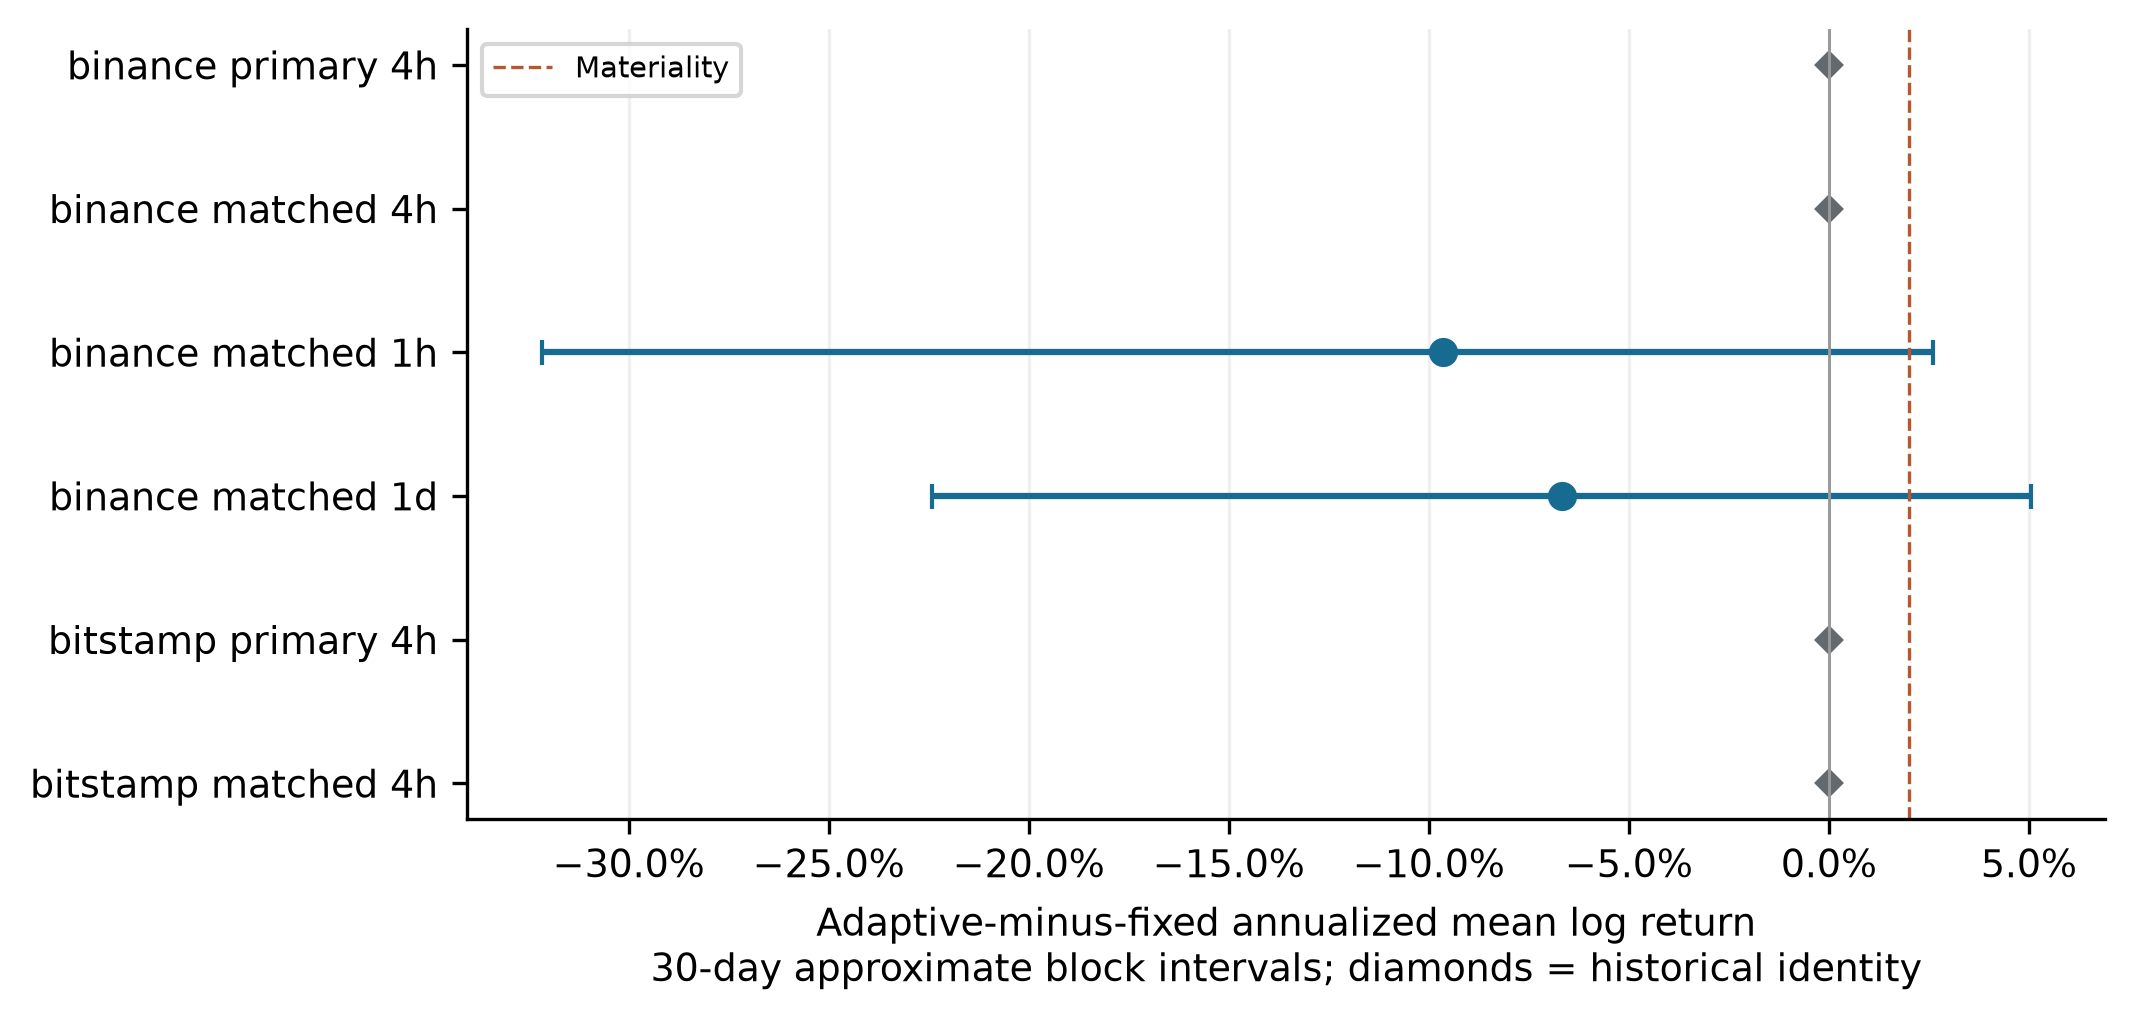
\includegraphics[width=\textwidth]{generated/market-paired-intervals.png}
\caption{All six prespecified application cases. Diamonds mark historical
identity. Intervals are not sequential or research-selection-adjusted evidence.
The dashed line is annual log materiality 0.02.}\label{fig:pairedmarket}
\end{figure}
